
\chapter{Software}
\label{Software}
\section{Arduino IDE on PC}
\label{Arduino IDE on PC}
\subsection{Installation}

Arduino Nano 33 BLE Sense can provide an energy-efficient and cost-effective solution for manufacturers who want to use Bluetooth Low Energy connectivity in their projects.\\

Arduino Nano 33 BLE Sense uses the Arduino software integrated development environment (IDE) for programming, which is the most widely used and common (IDE) for all arduino boards that can be run online and offline. This is a open-source Arduino Software (IDE) makes it easy to write code and upload it to the board. There are various version of software which is supported for each operating system (OS) e.g: mac, linux, and windows. Arduino community also provide us to start coding online and save our sketches in the cloud, this online arduino editor is most up-to-date version of the IDE includes all libraries and also supports new Arduino boards. For getting access to these software packages go to the following link \url{https://www.arduino.cc/en/software}  and get more up to date information, as there are frequent updates. These software can be used with any Arduino board, the most recent offline arduino IDE 2.0.3 can be seen in Figure, \ref{fig:arduino-creat-agent-installieren} it is also supportive for all operating systems.

\begin{figure}[h]
	\centering
	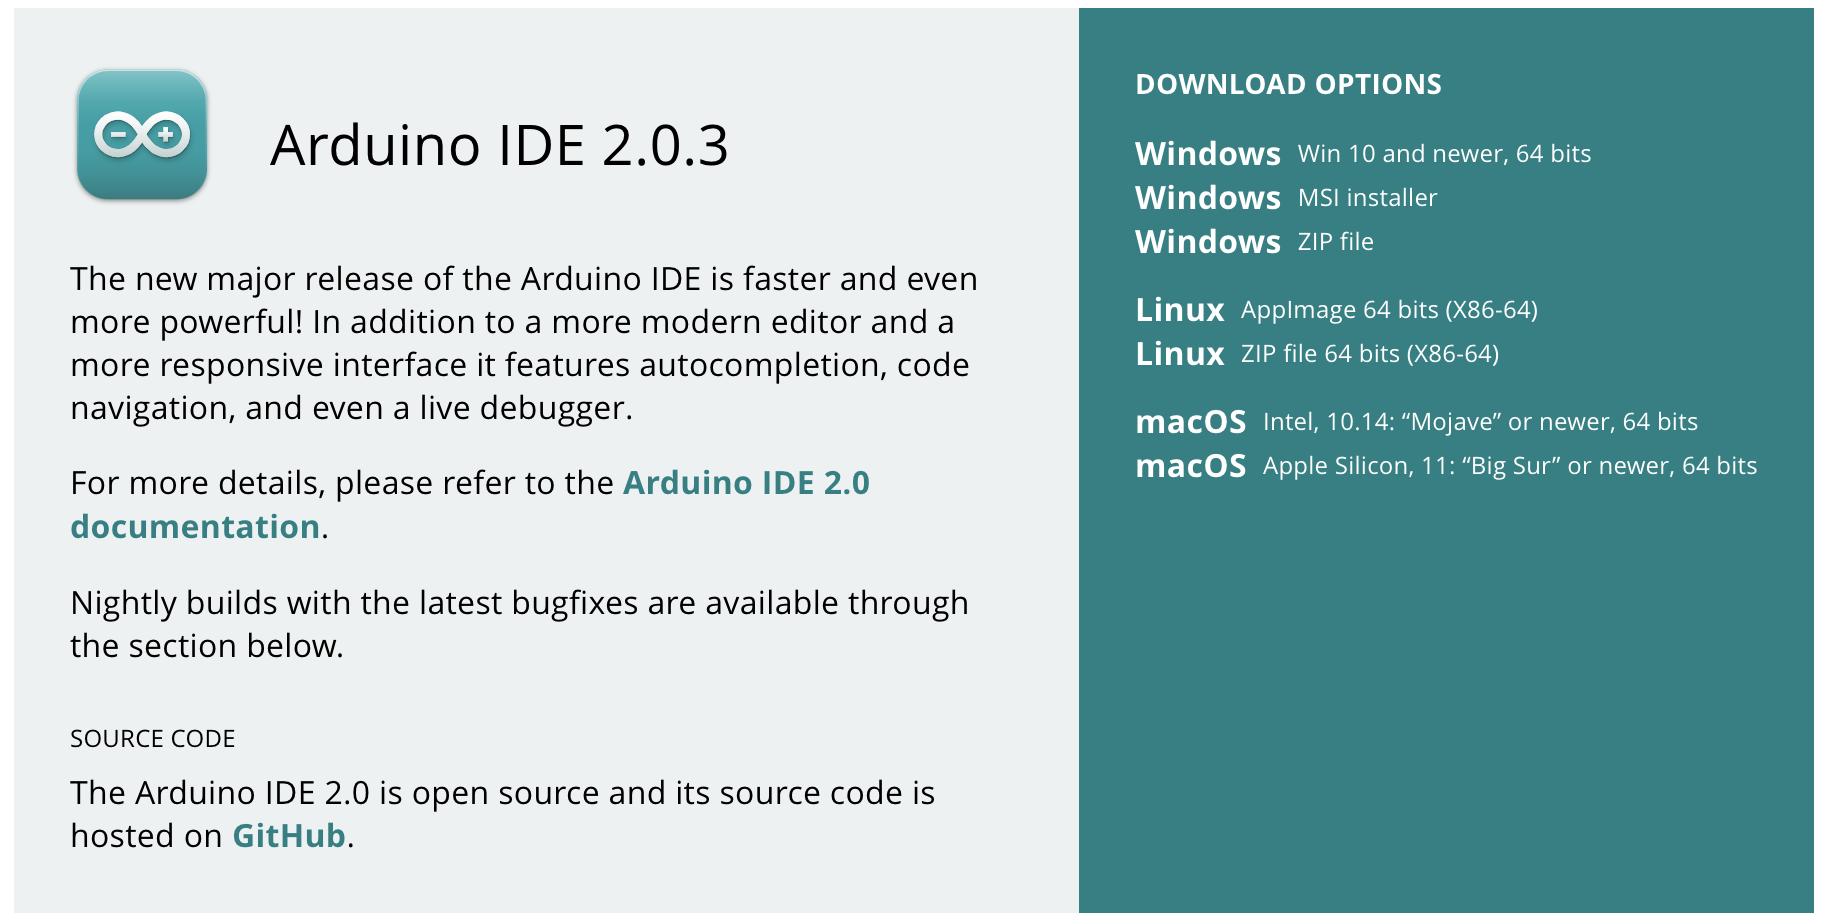
\includegraphics[width=1.0\linewidth]{Images/Arduino/Installation-1}
	\caption{Arduino Creat Agent Installation}
	\label{fig:arduino-creat-agent-installieren}
\end{figure}


\subsection{Configuration}

To program the Arduino Nano 33 BLE Sense in offline state, we need to install one of the latest arduino IDE on our desktop. After installation, for getting access to the Arduino Nano 33 BLE Sense board, we need to make configuration in our IDE. By opening the IDE, go to tool which can be seen on the uper left corner in IDE, in the tool there is an option for managed board. At this point we need to write our board name in the search which is Arduino Nano 33 BLE Sense as shown in figure, \ref {fig:Arduino-Mbed-Boards Installation} select the Arduino Mbed OS Boards and install it. The Mbed OS nano board supports also other nano family boards including Arduino nano 33 ble sense, after installing simply connect the Arduino Nano 33 BLE Sense to the computer via USB cable. 

\begin{figure}[h]
	\centering
	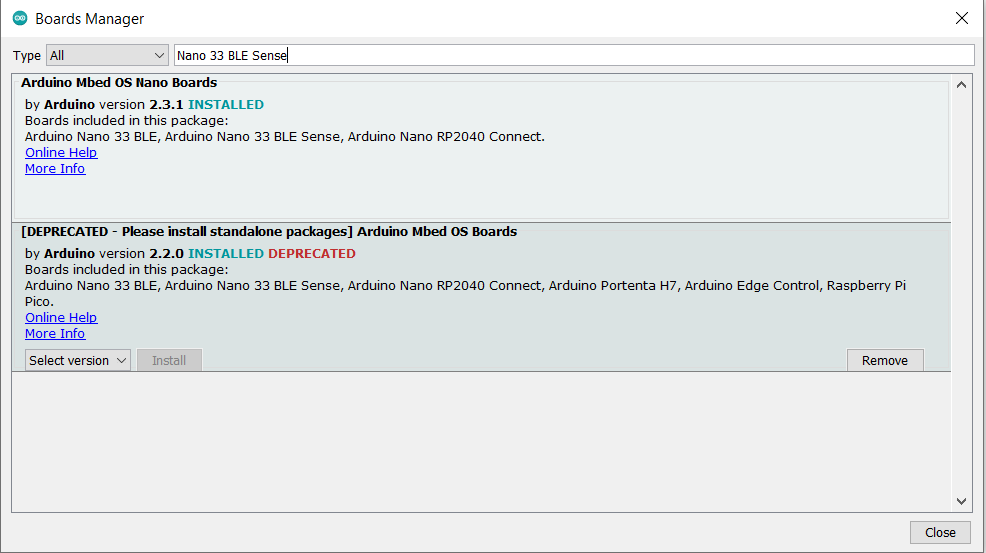
\includegraphics[width=1.0\linewidth]{Images/Nano33BLESense/Nano Mbed}
	\caption{Arduino Mbed OS Nano Boards Installation}
	\label{fig:Arduino-Mbed-Boards Installation}
\end{figure}


\subsection{Test Example}

There are set of examples which are build in Arduino (IDE) for the testing purpose, for checking all the configuration and setting up the board we can open one of the basic LED blink example first as shown in the figure \ref{fig:LED-Example}.

\begin{figure}[h]
	\centering
	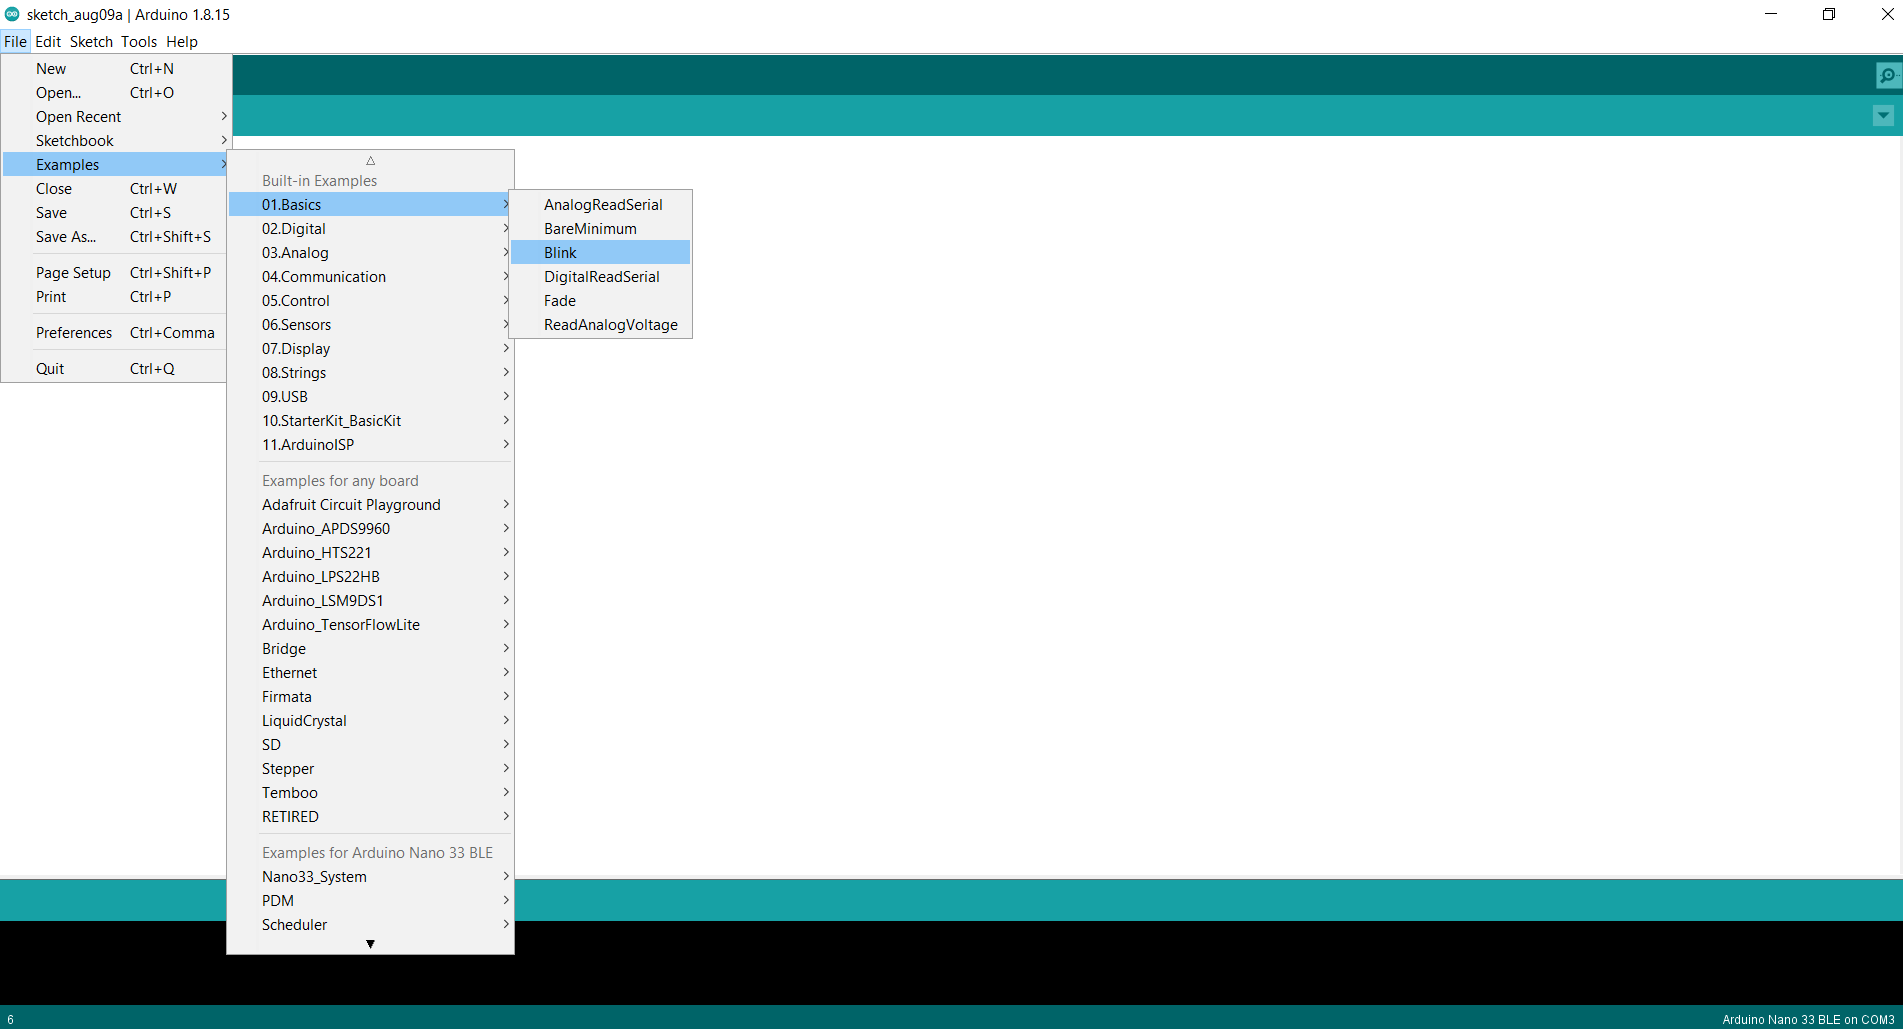
\includegraphics[width=1.0\linewidth]{Images/Arduino/LED}
	\caption{LED-Example Test}
	\label{fig:LED-Example}
\end{figure}

This LED-blink example support all the arduino boards, for the checking purposes just need to run this basic example on any arduino embed board and it will blink the LED on our Arduino board after pre-set miliseconds. In the same example folder, there are also number of build in usefull example written in Arduino IDE for embedded boards. These examples are very usefull for getting the basic knowledge about the board and programming.

\subsection{Pre-requisite settings for Uploading the program}
\label{Uploading the program} 
There are some pre-requisite steps need to follow either we need to run the build in example or run by our own written program. in order to program an Arduino board with a Laptop with the help of USB connection, open the Arduino IDE on desktop, a blank arduino environment page with just a Void setup and void loop written on it will appear. At this step we need to go to the tool-Arduino board and select the connected board which is Arduino Nano 33 Ble Sense as shown in the figure \ref{fig:Check Board}

\begin{figure}[h]
	\centering
	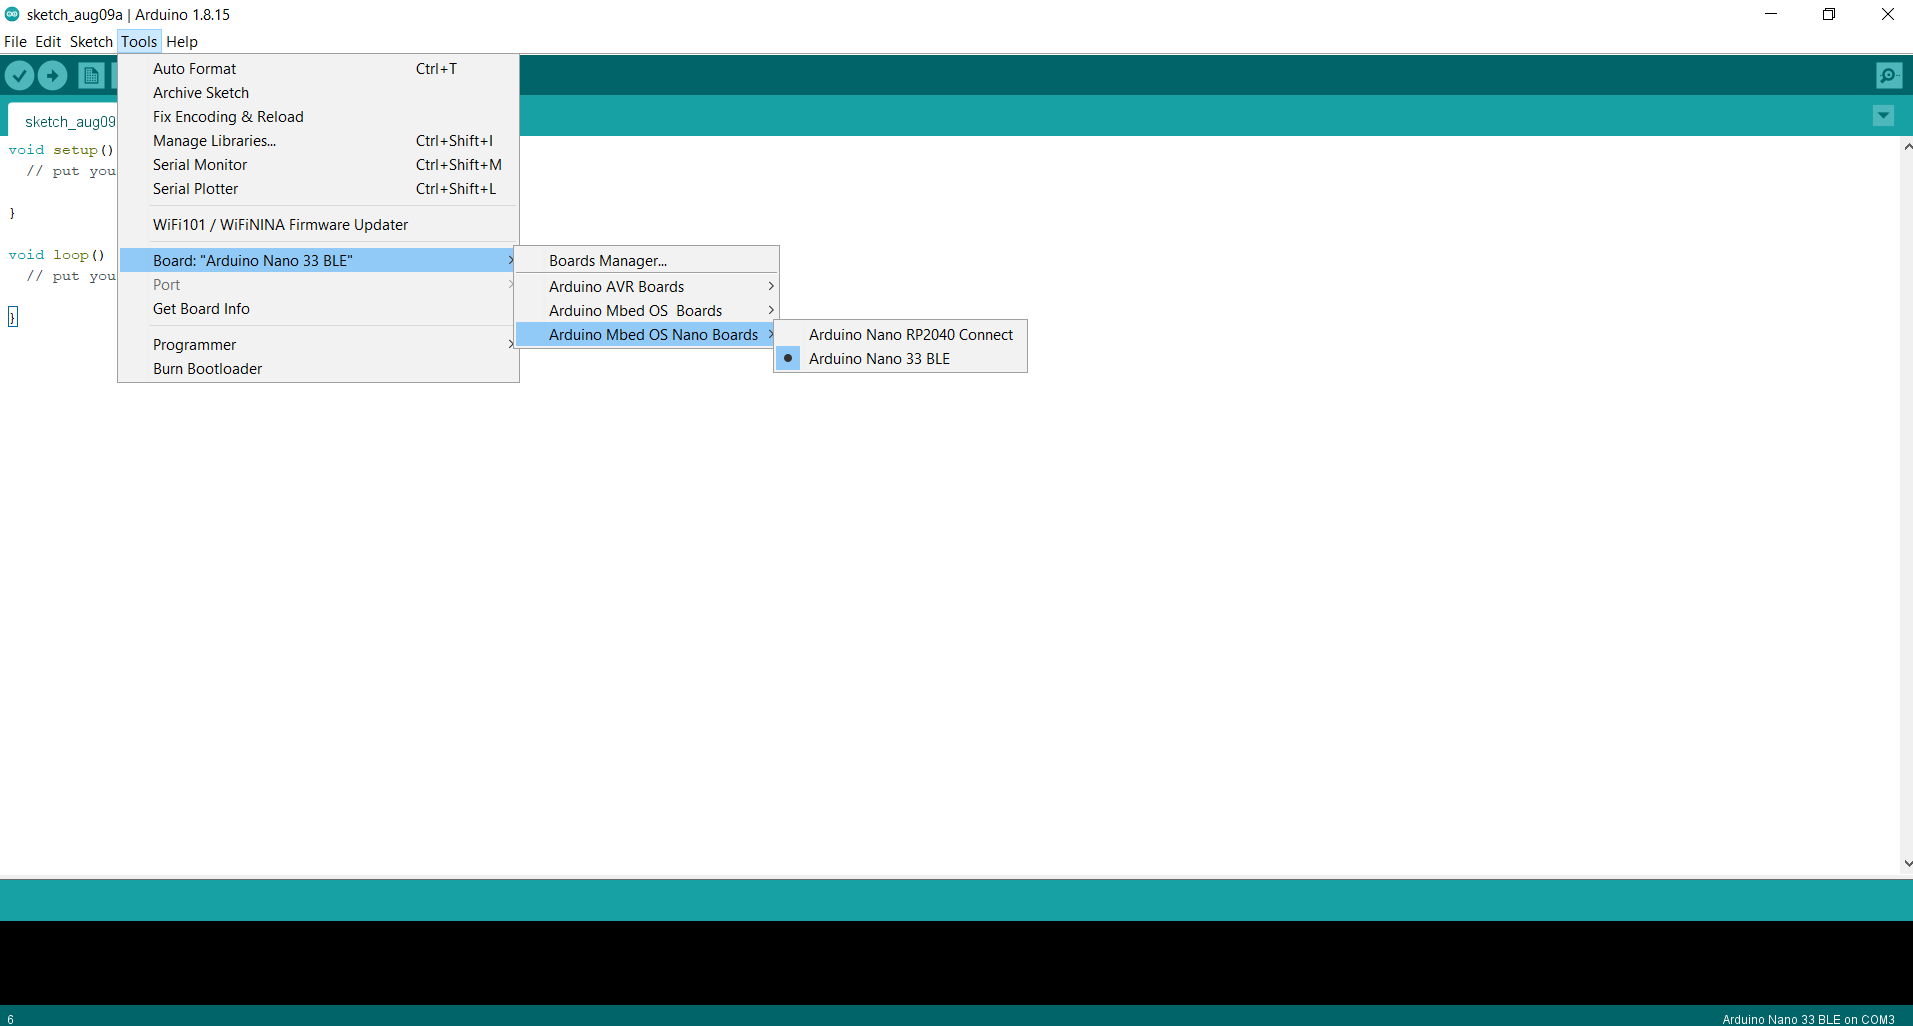
\includegraphics[width=1.0\linewidth]{Images/Arduino/Check-board}
	\caption{Select the Connected board}
	\label{fig:Check Board}
\end{figure}

\subsubsection{Select the Appropriate Port}

After selecting the Arduino nano 33 BLE sense board, next we need to check the connected port. For doing this, we need to set our arduino borad in Boot setup by clicking the white reset button on arduino as show in figure \ref{fig:Check-Reset}.

\begin{figure}[h]
	\centering
	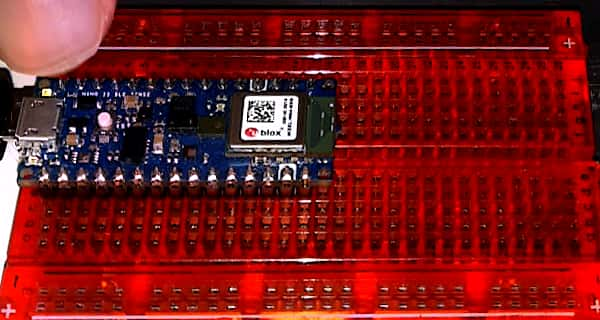
\includegraphics[width=1.0\linewidth]{Images/Arduino/Click-Reset}
	\caption{Reset Button}
	\label{fig:Check-Reset}
\end{figure}

By clicking the white reset button, the arduino borad will be in boot setup and make sure to check the orange LED glow as shown in the figure \ref{fig:LED-Glow}.

\begin{figure}[h]
	\centering
	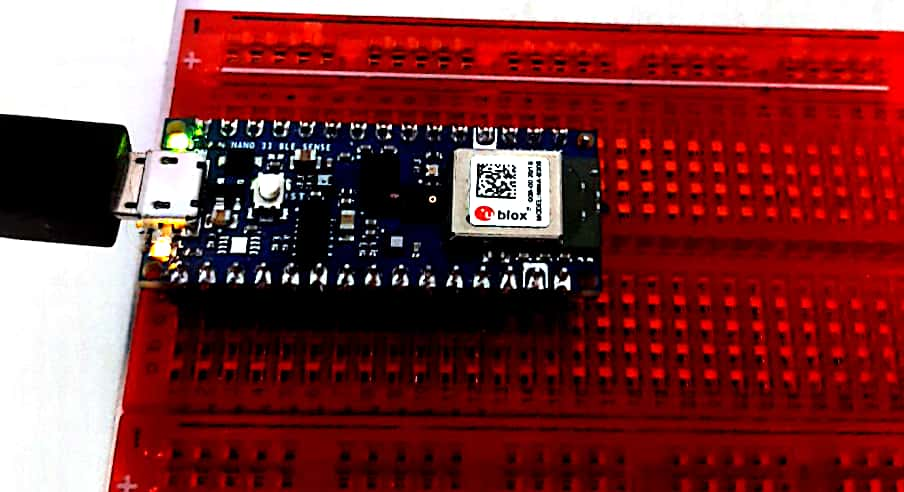
\includegraphics[width=1.0\linewidth]{Images/Nano33BLESense/Orange LED}
	\caption{Orange LED Glow}
	\label{fig:LED-Glow}
\end{figure}

After successfully applying the above mention step, next we need to select the connected port before upload the program. For this, go to tool select arduino port and make sure to check it available port for uploading the program as shown in figure \ref{fig:Port-Selection}

\begin{figure}[h]
	\centering
	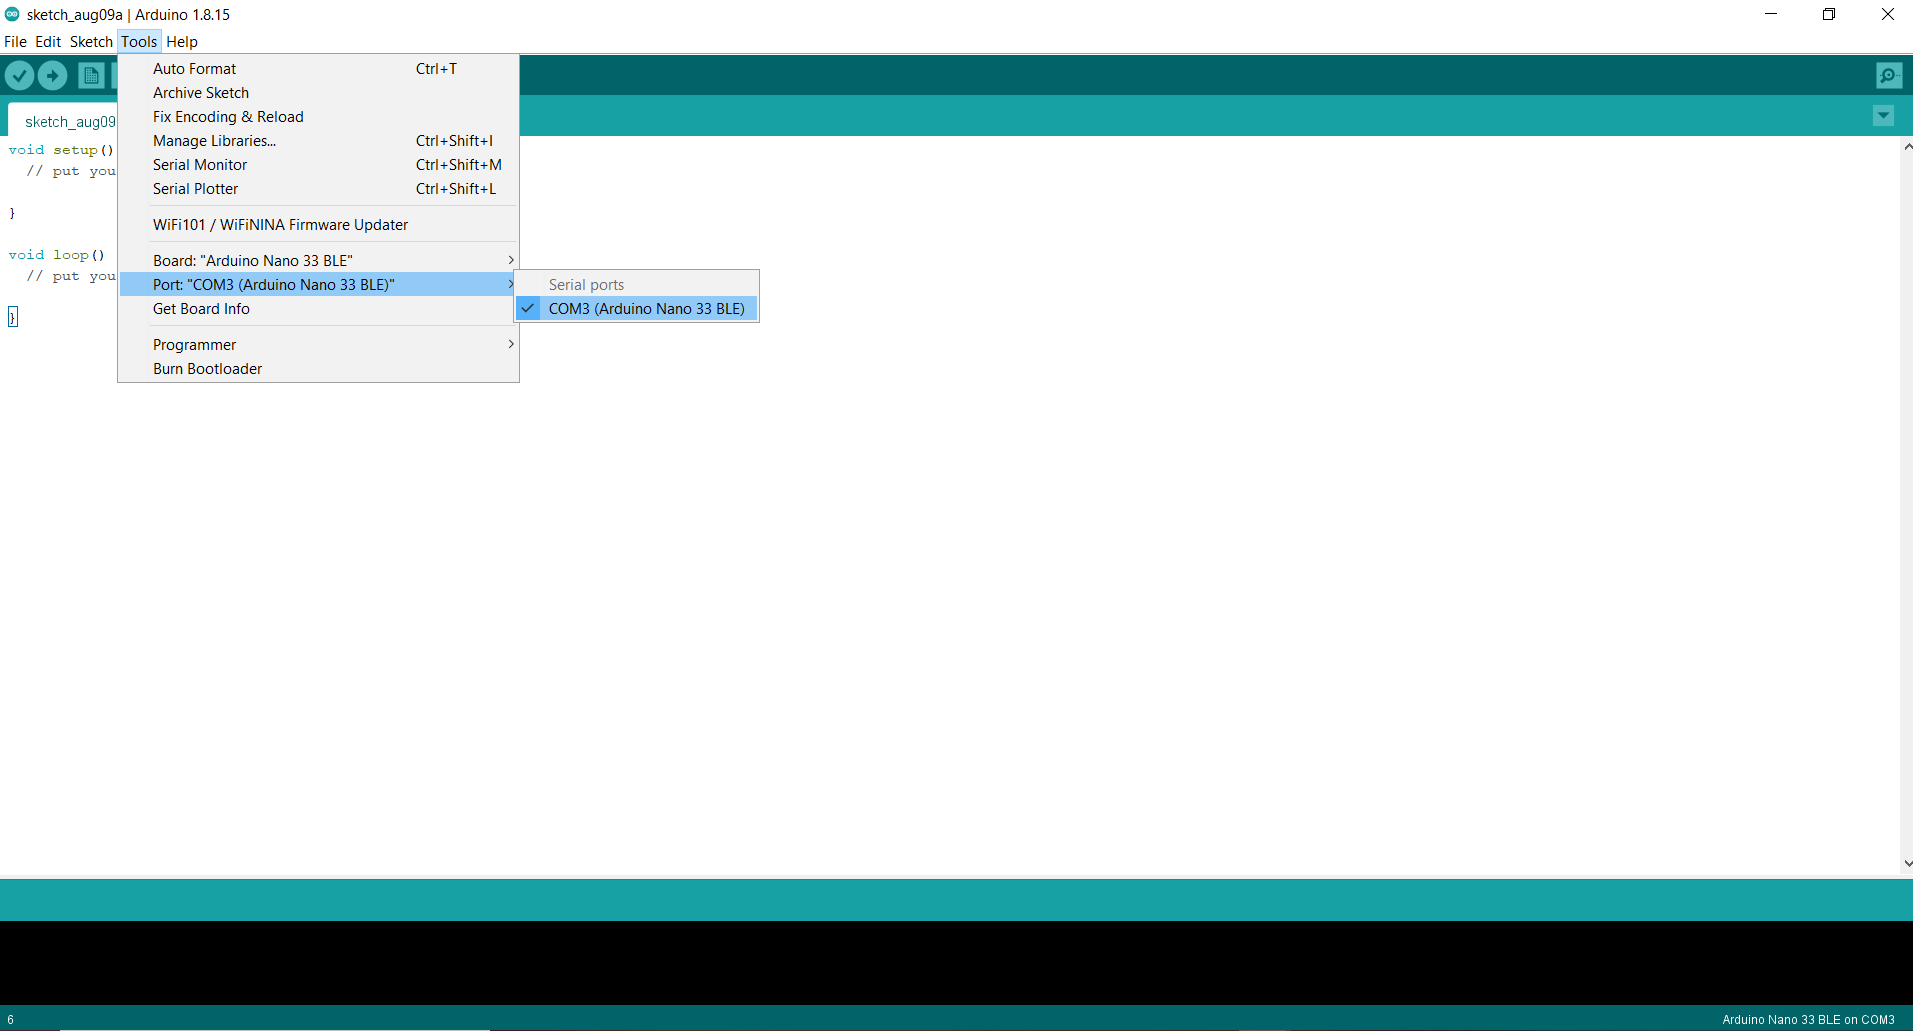
\includegraphics[width=1.0\linewidth]{Images/Arduino/Port-Select}
	\caption{Select Available Port for Uploading Arduino Sketch}
	\label{fig:Port-Selection}
\end{figure}

\subsubsection{Upload Code in Arduino Board}

After selecting the appropriate port, it's time to upload the Arduino program. There are five icons (verify, upload, new, open, save) below the file section, before uploading the program the best practice is to verify the program first, it show us if there are any error or warning in the program exist or not. By successfully verifying the program we can safely upload the program by click the upload button in the top below the file section as shown in figure. \ref{fig:Upload}.


\begin{figure}[h]
	\centering
	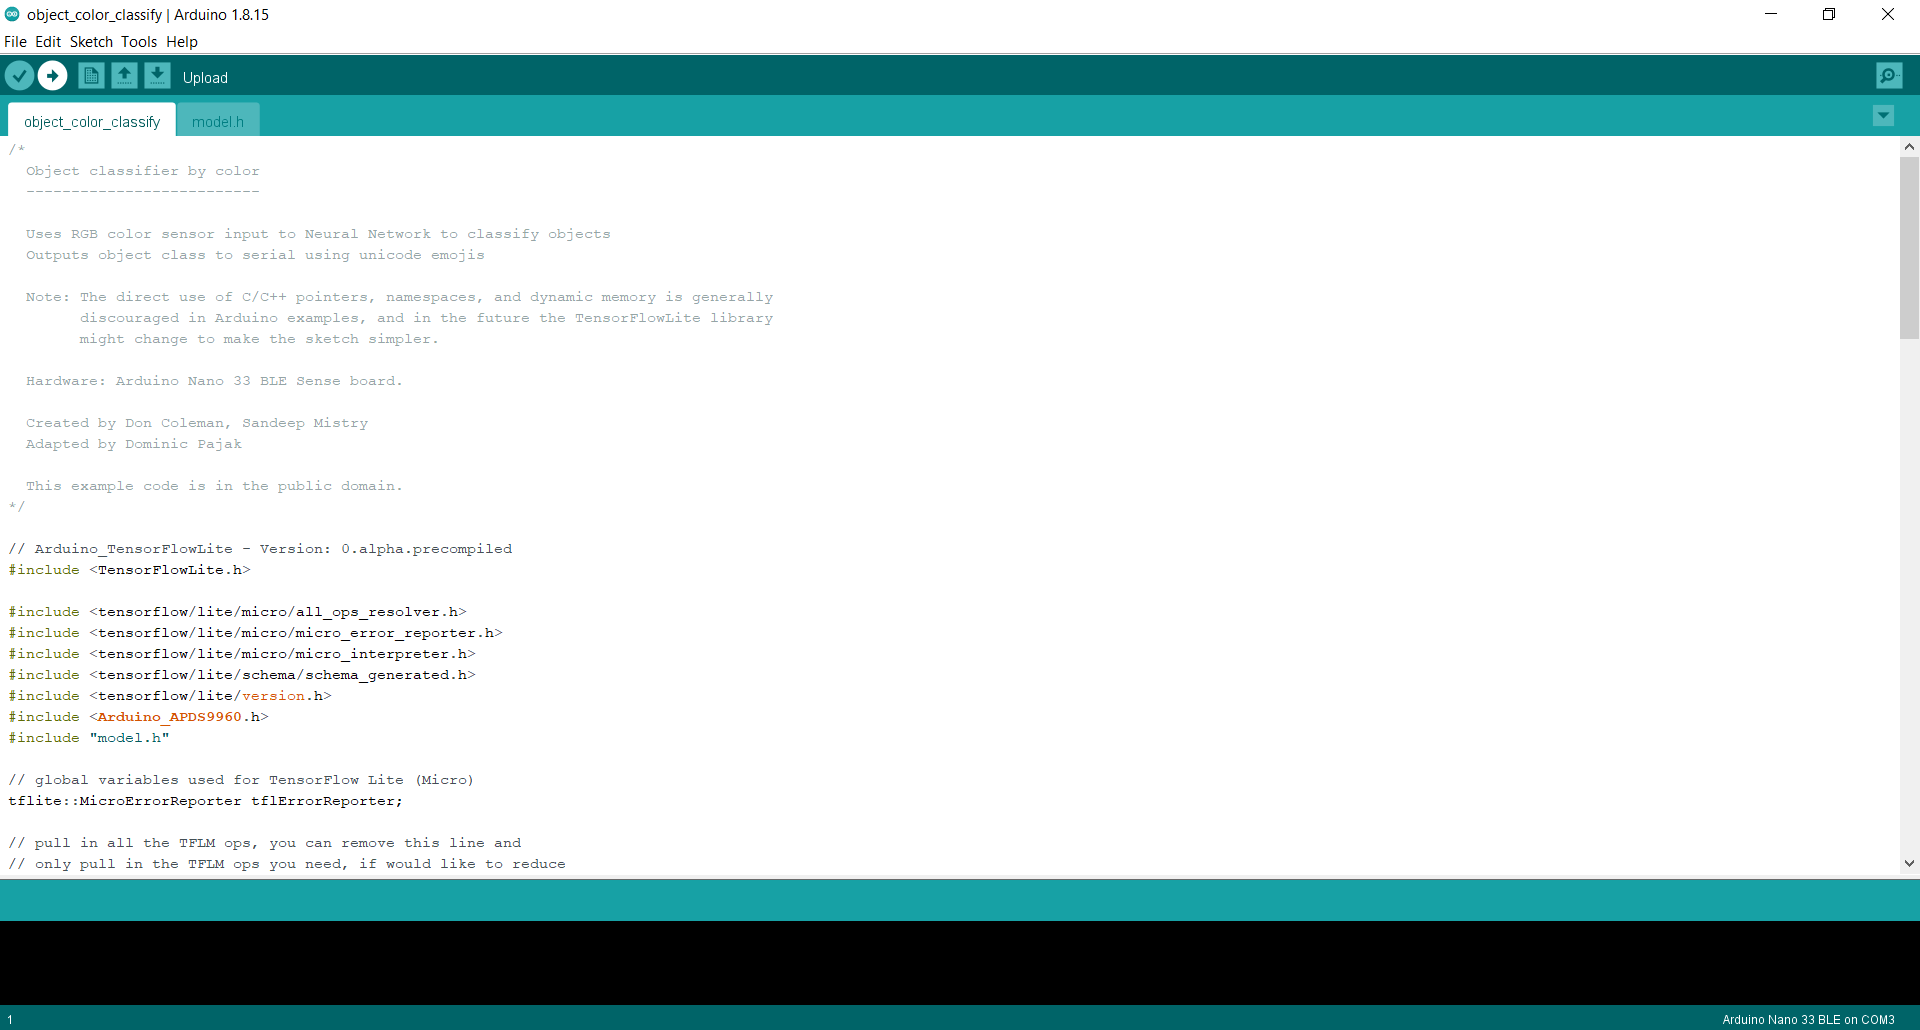
\includegraphics[width=1.0\linewidth]{Images/Arduino/Upload}
	\caption{Upload the Program in Arduino board}
	\label{fig:Upload}
\end{figure}

After uploading, the code will compile and if there is any issue in our program it will pop up in the bottom black window as well.

After successfully uploading and compiling the code in Arduino board, it also require to change the port again as we did it previously. Go to tool select arduino port and make sure to check the port again as shown in figure \ref{fig:Port} by getting output in the serial monitor.

\begin{figure}[h]
	\centering
	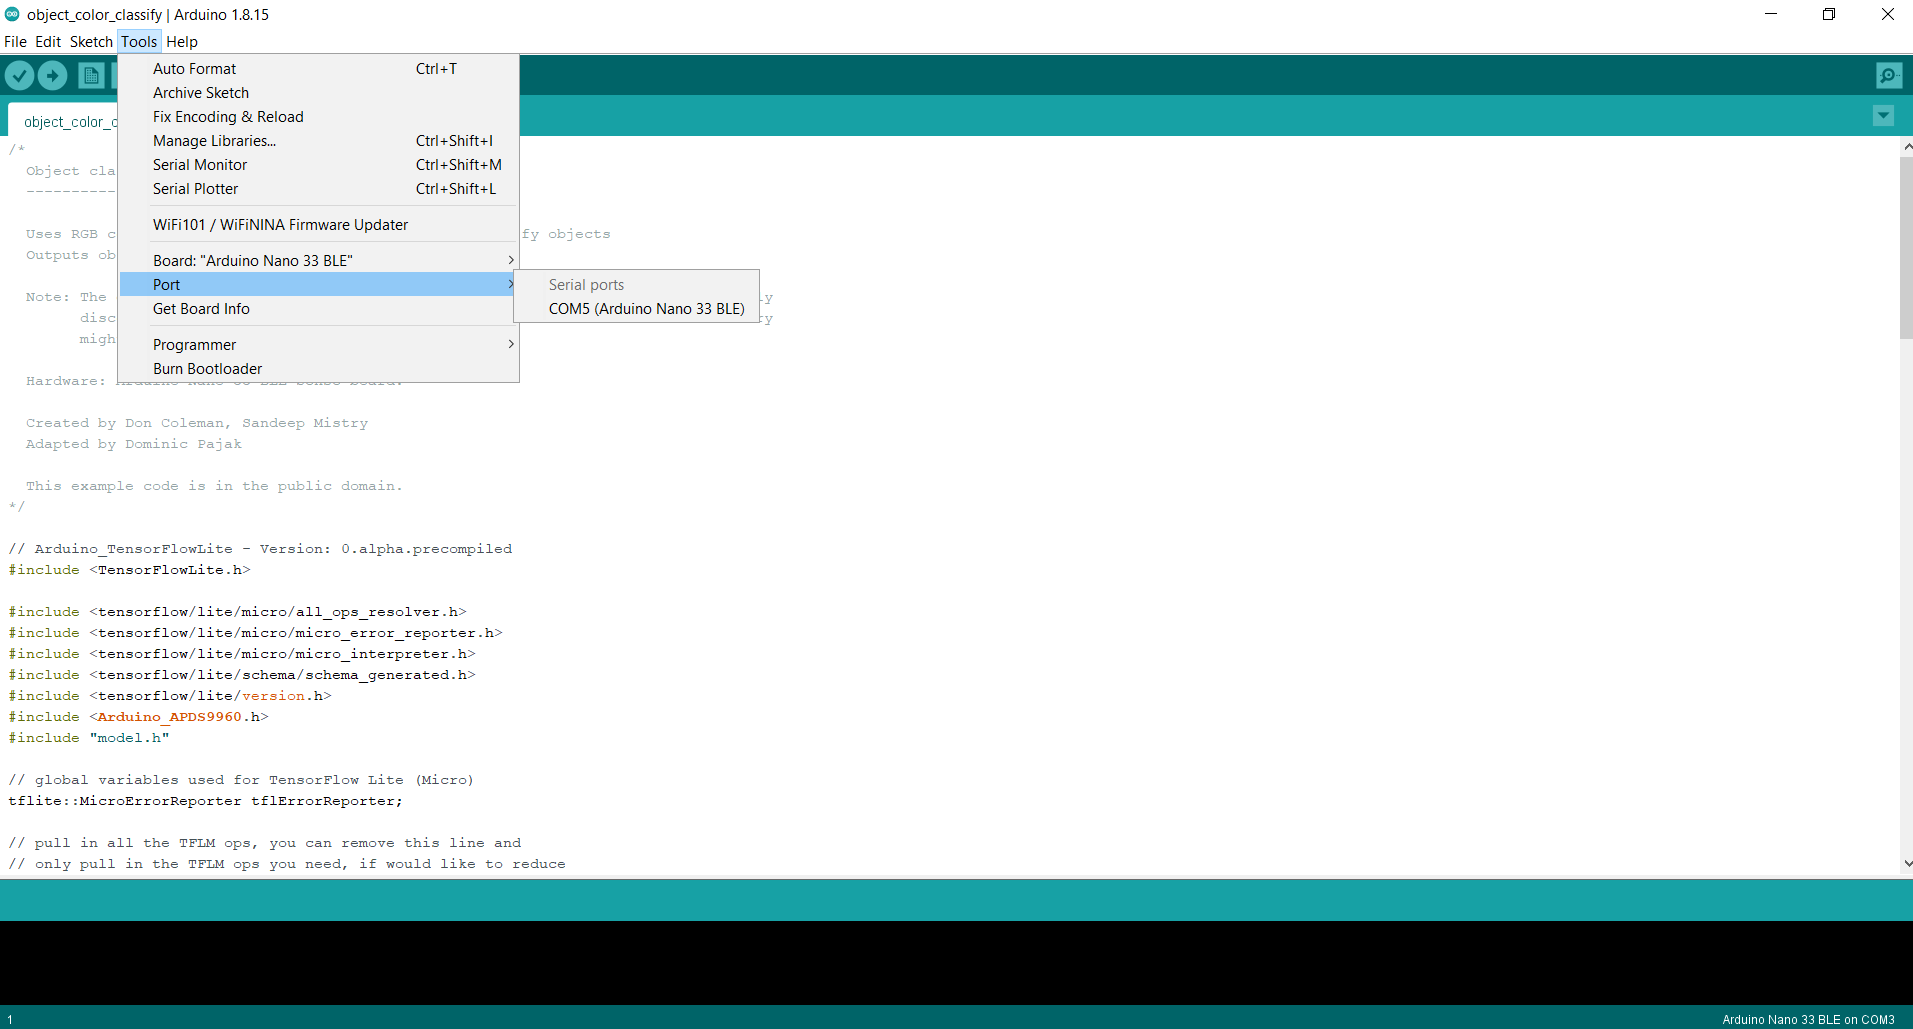
\includegraphics[width=1.0\linewidth]{Images/Arduino/Port}
	\caption{Setting the Port}
	\label{fig:Port}
\end{figure}

\section{Output Window (Serial Monitor)}

Serial Monitor is the another window on the Arduino IDE, which shows the Input/Output of our program and results appear on it as per the required output. For getting access to Serial monitor, we need to go extreme right in the Arduino IDE, the small circle pop up when we reach it is the serial monitor as show in the figure. \ref{fig:Serial Monitor}

\begin{figure}[h]
	\centering
	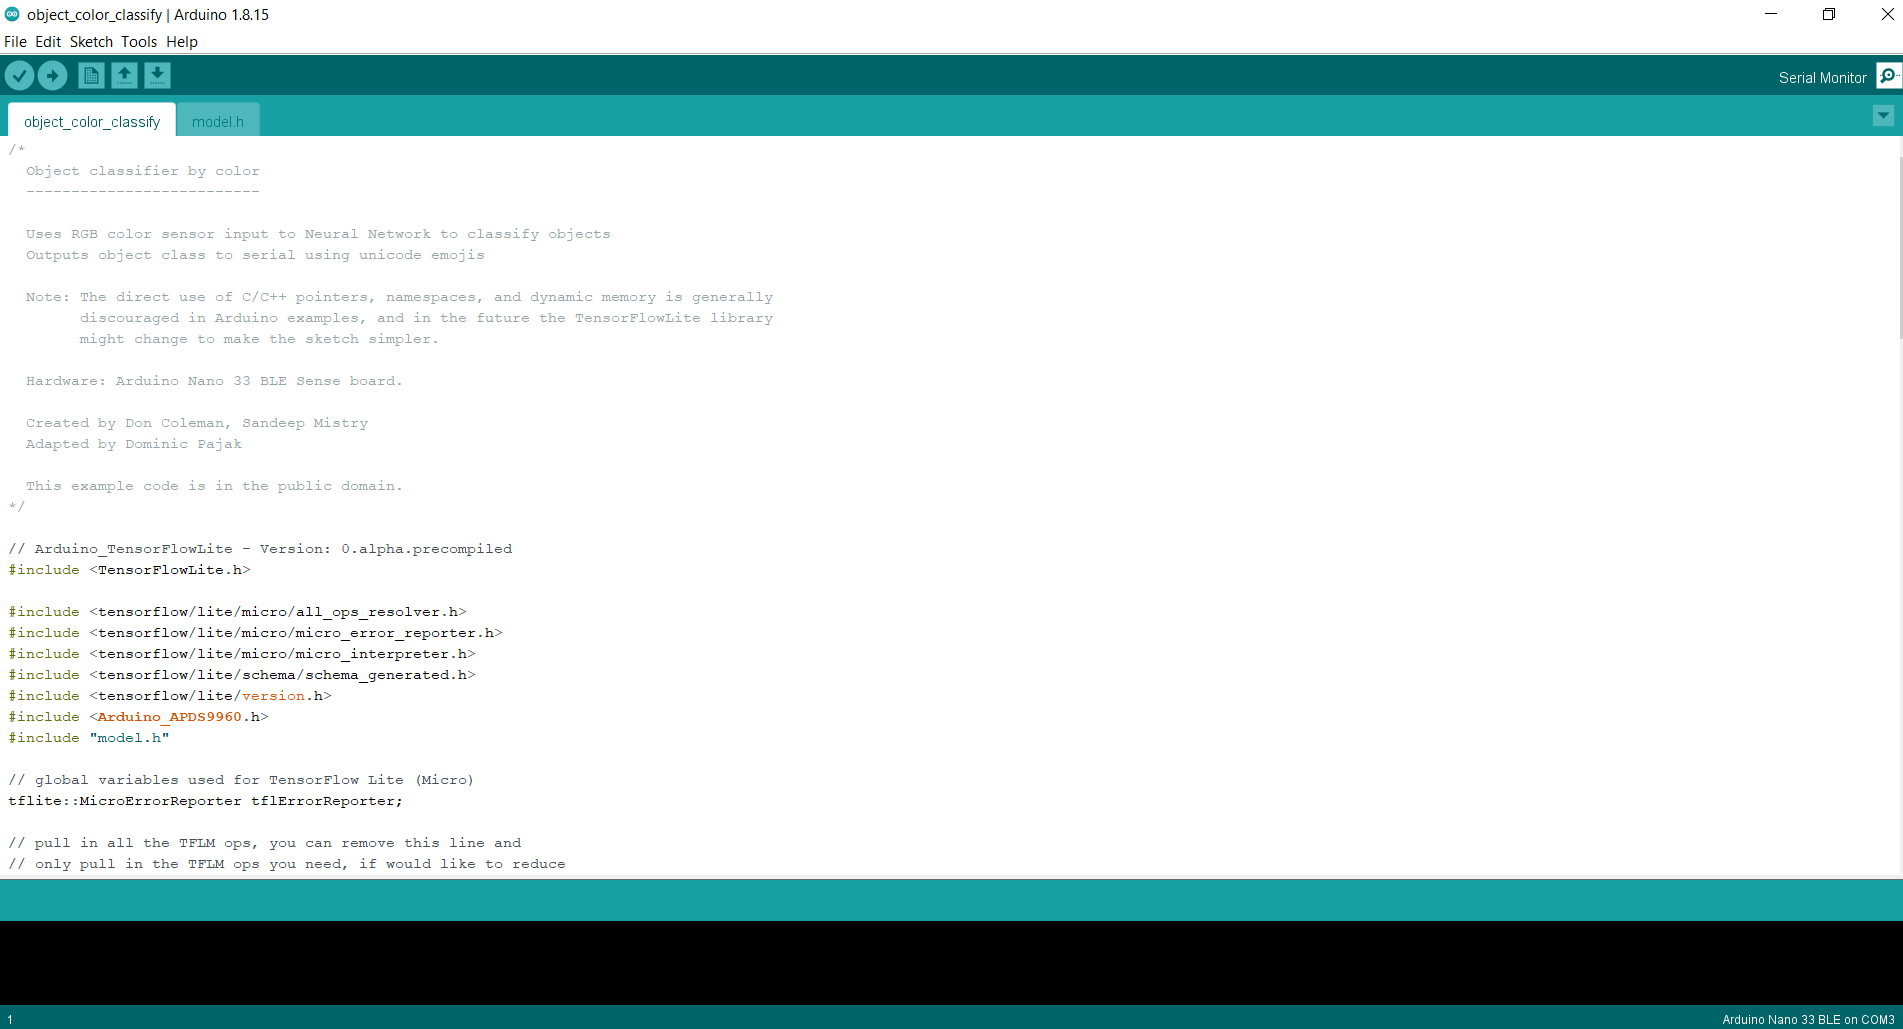
\includegraphics[width=1.0\linewidth]{Images/Nano33BLESense/Serial Monitor}
	\caption{Serial Monitor Icon}
	\label{fig:Serial Monitor}
\end{figure}

The Final results, all the variables, input, sensor values are shown in the serial monitor the (Output Window)  as shown in the figure \ref{fig:Output Window} by clicking the serial monitor button.

\begin{figure}[h]
	\centering
	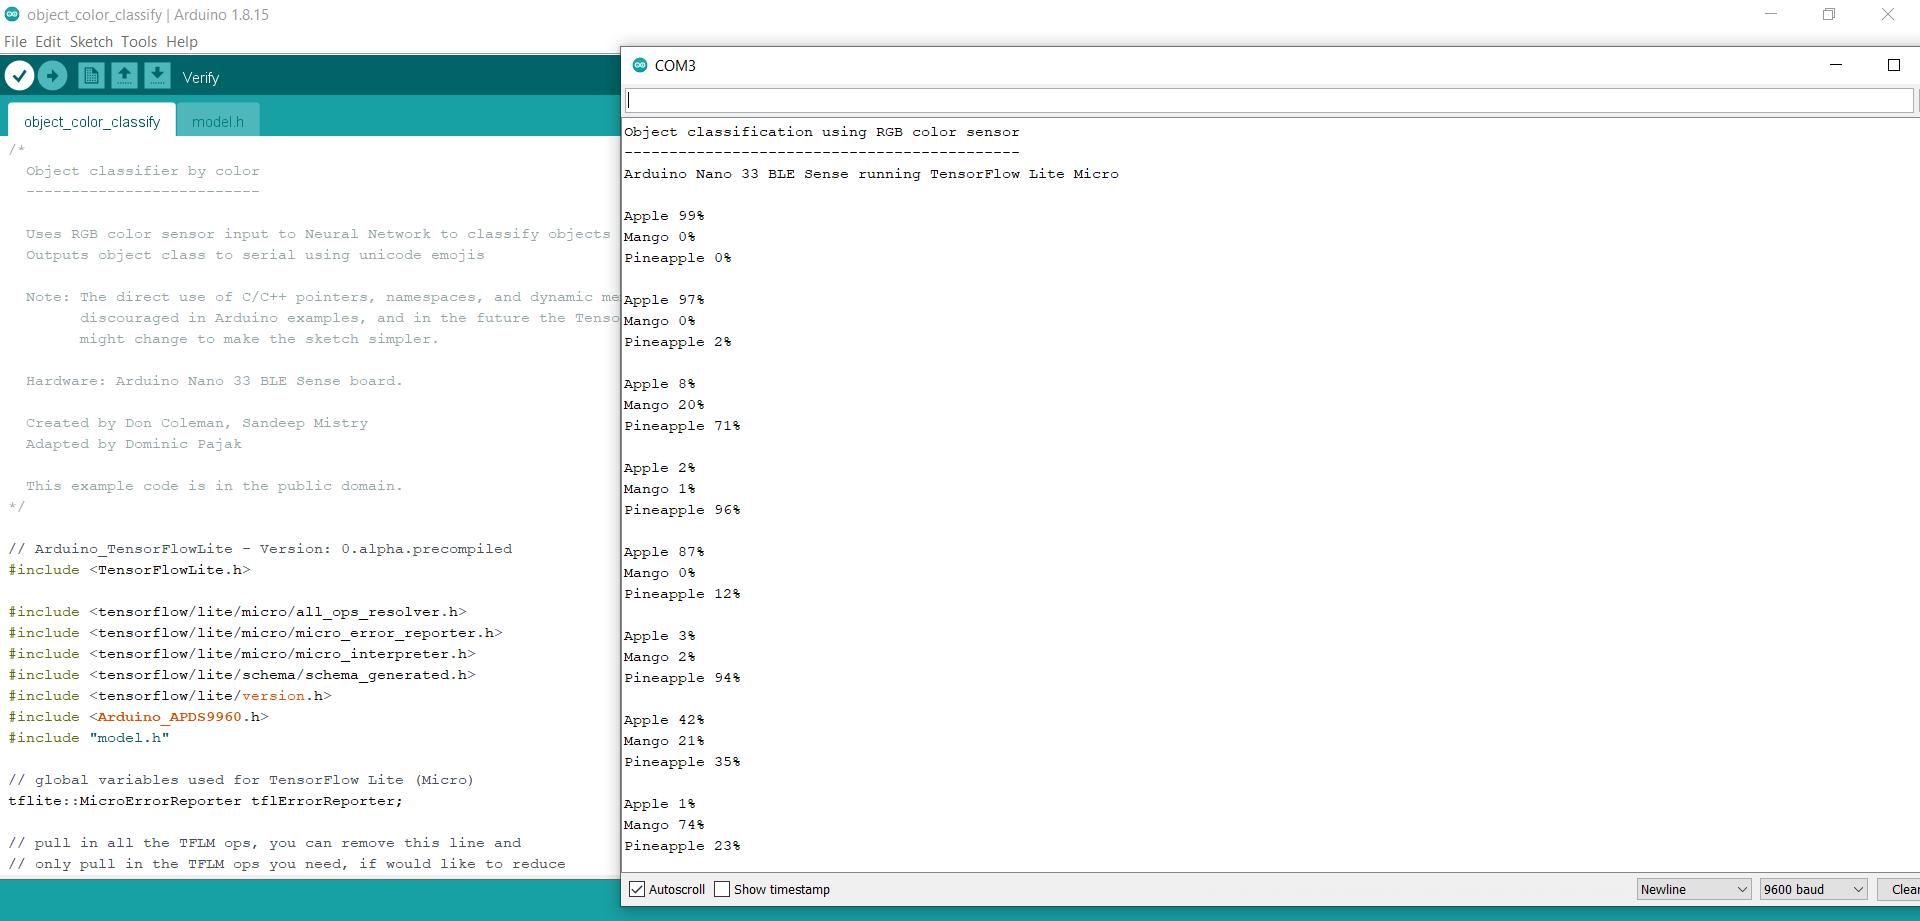
\includegraphics[width=1.0\linewidth]{Images/Nano33BLESense/4}
	\caption{Output Window}
	\label{fig:Output Window}
\end{figure}

%\section{Python on Pycharm}
%
%PyCharm is an integrated development environment (IDE) from the JetBrains company for the Python programming language. This Integrated development environment offers only the python programming environment, which will be usefull later in our project for running some computer vision python module.
%
%
%\subsection{Pycharm Installation}
%
%For getting up to date latest version of pycharm, we need to go \href{https://www.jetbrains.com/pycharm/download/#section=windows}{JetBrains-Link} and install the appropriate version as per our Operating system. 

%\section{Python Installation}
%
%Python is commonly used for developing websites and software, task automation, data analysis, and data visualization. Since it's relatively easy to learn, Python has been adopted by many non-programmers such as accountants and Data scientists, for a variety of everyday tasks, like organizing finances. It is an interpreted, object-oriented, high-level programming language with dynamic semantics. \href{https://www.python.org/downloads/}{Python Installation} at the time of writing this report the latest version of python is 3.9.7 release.\ref{Python Installation}
%
%\begin{figure}[h]
%	\centering
%	\includegraphics[width=1.0\linewidth]{Images/Arduino/python}
%	\caption{Python Installation}
%	\label{Python Installation}
%\end{figure}
%
%\section{Anaconda supporting framework for Jupyter Notebook}
%
%Anaconda is a distribution of the Python and R programming languages for scientific computing (data science, machine learning applications, large-scale data processing, predictive analytics, etc.), that aims to simplify package management and deployment. It is the most popular toolkit for data science environment. It support every package of Machine learning and Artificial Intelligence. The most widely used packages in machine learning are TensorFlow, OpenCV, and MediaPipe. the other supporting libraries include Numpy, Pandas, Matplotlib, Sklearn and many more. For getting up to date documentation and installation guide available at \href{https://www.anaconda.com/products/individual}{Jupyter notebook}. Anaconda support Jupyter notebook web application, it is the most widely used notebook for writing and training the Machine learning models.

\chapter{TensorFlow and TinyML}
\label{TFandTML}
\section{Machine Learning}
The integration of machine learning (ML) and artificial intelligence (AI) has become increasingly widespread, with applications spanning a wide range of industries and fields. These cutting-edge technologies are being employed to streamline processes and enhance accuracy, with some examples being their use in predictive maintenance within the manufacturing industry, transportation industry in Autonomous Vehicles for example in the Service sector Automated support processes,  \cite{McKinsey:2017}  and in medicine.

In the book "TinyML Machine Learning with TensorFlow Lite on Arduino and Ultra-Low-Power Microcontrollers," \cite{Warden:2020} the writers show that machine learning models can help to predict when a machine is about to break down. 
this is made possible by analyzing a collection of data on factors such as the machine's rate of production, temperature, and vibration.
this model made analysis make predictions about future states, helping to prevent damage before it even occurs.

In the transportation industry, AI is being leveraged to analyze road conditions and pave the way for the development of self-driving cars. In healthcare, the use of Machine Learning algorithms for the analysis of medical images, such as X-rays and CT scans, is becoming increasingly common. This is helping to improve the detection and diagnosis of diseases, such as cancer. Additionally, ML has also proven to be useful in predicting cardiac arrest, as demonstrated in a study from the journal Jmir medical informatics 2020 \cite{JMIR:2020}, which validated a developed model for clinical usefulness using data obtained from an electronic medical record hospital in the Emergency Department. The integration of these technologies has the potential to revolutionize the way we approach and solve problems, leading to improved efficiency and effectiveness across various fields..\cite{Dokic:2020}

Machine learning differs from traditional programming in that it relies on an algorithm to discover the relationships in the data and build a model for making predictions, rather than explicitly coding the rules. traditional coding may work just fine in many cases for example, we know that water boils at 100°C at sea level, so it’s easy to write a program that can predict whether water is boiling based on its current temperature and altitude. this may however be problematc if the cause is a combination of various factors. and this is when maschine learning is needed as it allows for predictions to be made based on complex data without the programmer having to understand all the details.  \cite{Warden:2020}	

\section{TensorFlow}

TensorFlow is an open-source deep learning library developed by the Google Brain team in 2015. It is widely used for creating, training, evaluating, and deploying machine learning models \cite{Warden:2020} . 

TensorFlow provides APIs in various programming languages such as Python and C++, making it easy to use for a wide range of applications. While TensorFlow can be used for traditional machine learning tasks, it is particularly powerful for developing complex deep learning applications such as text and image recognition.  \cite{Rajendra:2021} . 

\subsection{TensorFlow Features}
\begin{itemize}
	\item Auto Differentiation: TensorFlow provides automatic differentiation capabilities, which allow you to easily calculate gradients of a function with respect to its inputs. This is useful for training machine learning models using gradient-based optimization algorithms.
	\item Flexible computation: TensorFlow allows you to perform computations on a variety of devices, including CPUs, GPUs, and TPUs. This makes it easy to scale your computations and take advantage of the available resources.
	\item Large ecosystem: TensorFlow has a large ecosystem of tools and libraries, including TensorFlow Lite and TensorFlow.js, that can be used to perform a wide range of tasks such as training, deploying, and monitoring machine learning models.
	\item Portability: TensorFlow models can be deployed on a wide range of platforms, including mobile devices, web browsers, and servers. This allows you to easily deploy your models in a variety of environments.
	\item Support for multiple languages: TensorFlow provides APIs in multiple languages such as Python, C++, and Java, making it accessible to developers of all skill levels.
	\item Visualization: TensorFlow provides built-in support for visualizing your models and data, which can help you understand and debug your models.
	\item Easy model deployment: TensorFlow provides tools for deploying models to a variety of platforms, including mobile devices and web browsers.
\end{itemize}

\subsubsection{Usage and extensions}
TensorFlow is both the core platform and a library that one can use for machine learning purposes, Keras an open-source software library written in Python, acts as an interface for the TensorFlow library to make creating machine learning models easier.
\url{https://www.tensorflow.org/guide/basics}
%\subsubsection{Applications}
%https://datasolut.com/einfuehrung-in-tensorflow/
\subsubsection{Limitations of TensorFlow}

Tensorflow can not be used in mobile phones or embedded devices because of their limited memory, to avoid this inconvenience, Google also developed TensorFlow Lite, a tool that makes it possible to use already trained models on smaller memory devices.

\url{https://www.tensorflow.org/lite/guide}

\section{TensorFlow Lite}
%general
TensorFlow Lite is a streamlined version of TensorFlow designed for mobile and embedded devices, enabling machine learning inference to be performed directly on the device \url{https://www.tensorflow.org/lite/guide} with minimal latency and a small binary size. its models can be recognised by the .tflite file extension, and is represented in a special efficient portable format known as FlatBuffers.

in order for it to achieve low latency, TensorFlow Lite implements a range of techniques, such as optimizing kernels specifically for mobile applications, using pre-fused activations, and quantized kernels that allow smaller and faster models.
TensorFlow Lite also supports hardware acceleration through integration with the Android Neural Networks API. 

To generate a TensorFlow Lite model, there are in general three possible ways and thus:
\begin{itemize}
	\item By using existing TensorFlow Lite models from a selection of pre-trained TensorFlow Lite models developed for specific cases.
	\item By using the TensorFlow Lite Model Maker in order to create a model with a specific custom dataset. 
	\item By Converting a trained TensorFlow model into a TensorFlow Lite model using the TensorFlow Lite Converter.  
	
\end{itemize}
in this chapter, however, we will only focus on the third way; Converting an existing model to a TensorFlow Lite model specifically in \ref{Convert the model with TensorFlow Lite}.
%Architecture

In Fig \ref{TensorFlow Lite Architecture}, you can see the architecture of TensorFlow Lite. Once you have a trained TensorFlow model, it is converted to a TensorFlow Lite model file (tflite) using a converter. This conversion process optimizes the model for mobile devices, making it smaller and faster to run.

After the model is converted to a tflite file, it can be used to create either an Android or an iOS app. This means that your powerful machine learning model can now be integrated seamlessly into a mobile app, making it available to users on the go.

TensorFlow Lite offers a range of useful features that make it a great choice for developing machine learning models for mobile platforms. These include:

\begin{itemize}
	\item Core operators: TensorFlow Lite includes a collection of core operators that are compatible with both quantized and float formats, making it easy to deploy models on mobile devices.
	
	\item Mobile-optimized interpreter: The new interpreter in TensorFlow Lite is specifically designed to keep mobile apps fast and lean, and it includes a less dynamic memory allocator that minimizes load utilization.
	
	\item Hardware acceleration: TensorFlow Lite also supports hardware acceleration using the Android Neural Networks API. This enables models to run even faster on supported devices, improving performance and reducing latency.
\end{itemize}
\begin{figure}
	\centering
	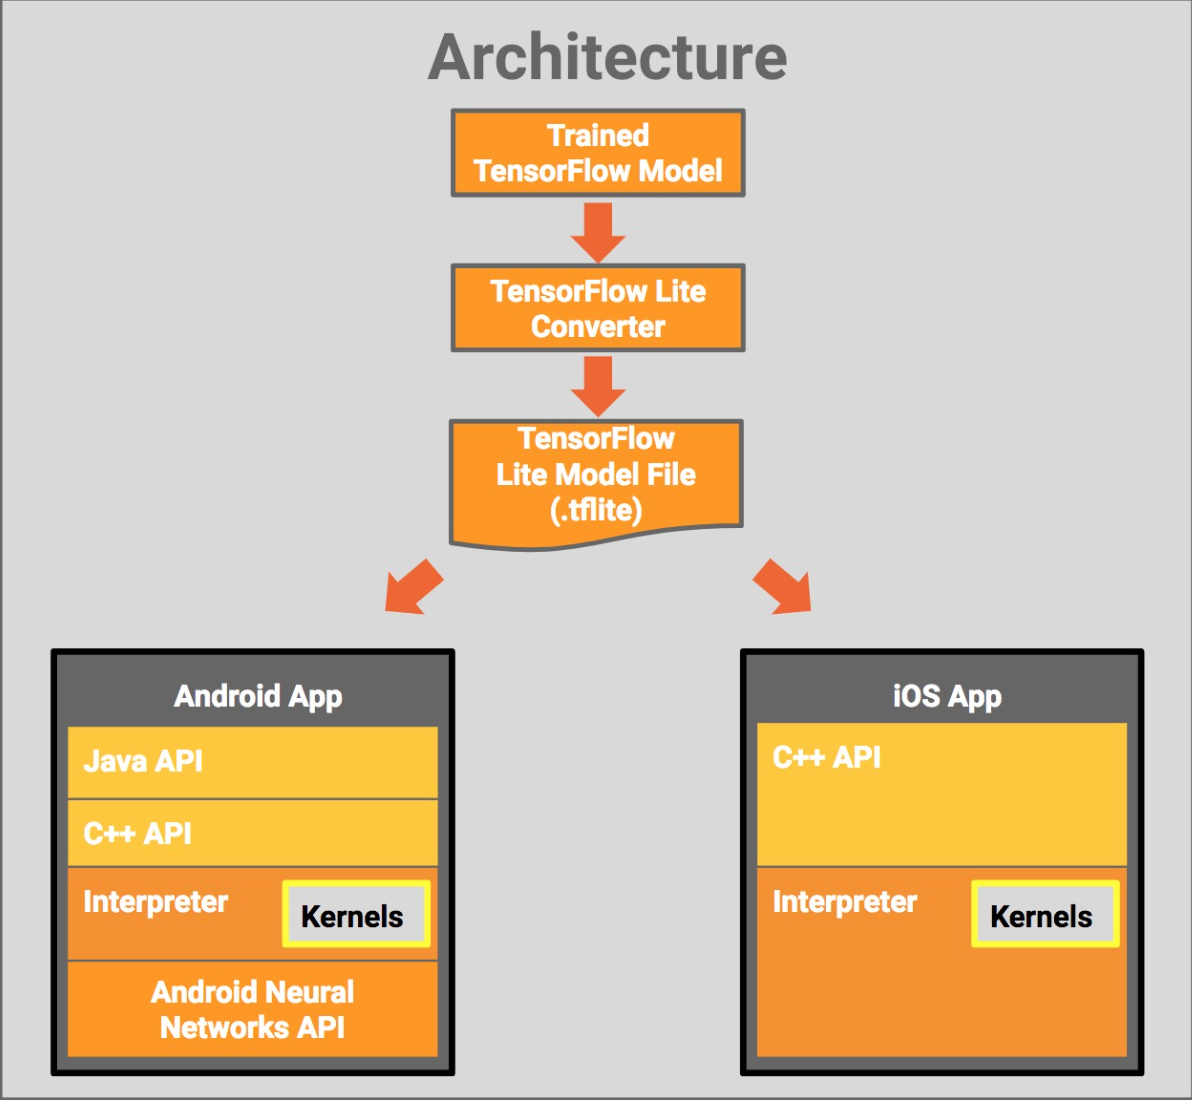
\includegraphics[width=0.5\textwidth]{Images/TF Lite Architecture}
	\caption{TensorFlow Lite Architecture: www.tensorflow.org}
	\label{TensorFlow Lite Architecture}
\end{figure}

Overall, TensorFlow Lite is a powerful tool that enables you to take your trained machine learning models and use them in mobile apps, bringing the benefits of machine learning to a wider audience however it still has its limits.

\subsubsection{Limitations of TensorFlow Lite}
in order to efficiently run machine learning models on embedded devices and mobile phones, certain compromises need to be made. 
these include the inability to train models directly on the device, and the requirement that inference can only be run on models that were previously trained on another device or in the cloud (See \ref{TensorFlow Lite Architecture}).
Furthermore, certain data types such as doubles may not be available, and some less frequently used functionalities may be absent \cite{Warden:2020}. These trade-offs enable the model size to be reduced, making it possible to incorporate the model into devices with limited memory space.
\subsection{TensorFlow Lite for microcontroller}
\url{https://www.hackster.io/theevildoof/how-to-get-started-with-tensorflow-lite-for-microcontrollers-f0c884#:~:text=TensorFlow%20Lite%20Micro%2FTinyML%3A%20TensorFlow,libraries%2C%20or%20dynamic%20memory%20allocation.}
\ref{David:2021}
\subsection{TinyML and Real Time}

The device we are developing requires real-time processing of a person's movement to deliver the wished result. 
However, the utilization of TinyML systems presents several challenges in achieving this level of performance. The limited computational power and memory of our Arduino nano 33 BLE sense make it difficult to run complex machine-learning models in real time, and the storage and processing of large amounts of data can further impede real-time performance. 
Despite these challenges, it is still feasible to achieve real-time processing using TinyML systems by implementing certain approaches. 
One approach is to utilize machine learning models that are better suited to the limited resources of TinyML devices.
Additionally, techniques such as model quantization, pruning, and compression can be employed to optimize and simplify the model, making it more efficient and better suited to the limitations of the device.
Edge computing and on-device processing can also be utilized to reduce the amount of data that needs to be transmitted, stored, and processed, further enhancing real-time performance.
\section{TinyML Workflow}

\textcolor{red}{TinyML and Real Time}
\textcolor{red}{TinyMLWorkflow}
\textcolor{red}{Workflow}  
\textcolor{red}{TensorFlow Lite} 	\textcolor{red}{TensorFlow Micro} 
%General
TinyML pertains to the implementation of machine learning algorithms on small, low-power devices such as microcontrollers and sensors \cite{David:2021}, with an example being the Arduino Nano 33 BLE Sense. 
TinyML models are capalbe of on-device analytics for a variety of sensing modalities (vision, audio, speech, motion, chemical, physical, textual, cognitive) at mW (or below) power range setting. \cite{Ray:2021}
%



\subsection{choice of Algorithm}
In order to develop a ML application we first need to choose the machine learning model that suits the our needs and thus, based on the type of data we are working with, in our case the WISDM dataset (see Chapter \ref{Datasets} for more details),and the requirements of the deployment environment or the constraints of the Arduino board we will be working with. 
We already have three possible algorithms we can work with, these are portreted in more detail in charpter \ref{Algorithms} .
\subsection{Train the model}


\subsection{Convert the model with TensorFlow Lite}
%TensorFlow Lite workflow
\label{Convert the model with TensorFlow Lite}

%in this chapter, however, we will only focus on the third way; Converting an existing model to a TensorFlow Lite model.

Lets say we have developped and trained a model with TensorFlow and now we want to use it on our Arduino board.
in order to do so the trained model needs to be converted to a compatible format with small devices. 
Here the step by step guide for conversion into TensorFlow Lite assuming we already have a trained TensorFlow model:

First step is to make sure both TensorFlow and TensorFlow Lite are installed 
Second we need to load the trained TensorFlow model using tf.saved\_model.load() function. .
import tensorflow as tf
\lstset{language=Python}
%\begin{lstlisting}
\begin{verbatim}
	import tensorflow as tf
	# Load the trained TensorFlow model
	model = tf.keras.models.load_model('path/to/saved_model')
\end{verbatim}
%\end{lstlisting}

Then we have to start converting the TensorFlow model to TensorFlow Lite using the TensorFlow converter fuction: 


\begin{verbatim}
	# Convert the model to TensorFlow Lite format
	converter = tf.lite.TFLiteConverter.from_saved_model('path/to/saved_model')
	tflite_model = converter.convert()
\end{verbatim}


After the conversion we need to save our TensorFlow Lite model to a file using the open() and write() functions
\begin{verbatim}
	# Save the model to a file
	with open('model.tflite', 'wb') as f:
	f.write(tflite_model)
\end{verbatim}

And as final step, the coverted TF lite model is now tested using the tf.lite.Interpreter() class. this step helps us see if the created model has lost its accuracy.
\begin{verbatim}
	# Load the model
	interpreter = tf.lite.Interpreter(model_path='model.tflite')
	
	# Allocate memory for the model
	interpreter.allocate_tensors()
	
	# Get input and output tensors
	input_details = interpreter.get_input_details()
	output_details = interpreter.get_output_details()
	
	# Test the model
	input_data = # Provide input data in the required format
	interpreter.set_tensor(input_details[0]['index'], input_data)
	interpreter.invoke()
	output_data = interpreter.get_tensor(output_details[0]['index'])
\end{verbatim}
\subsection{Optimize the model}
To compress the TensorFlow lite model even more and gain on space there some optimization possibilities available, two of them being: 
\begin{itemize}
\item Quantization: which consists in converting floating-point values to fixed-point values. You can choose between full-integer quantization or float-16 quantization.
\item Pruning: a technique that removes the weights with the smallest magnitude from the model

\end{itemize}
in case we used compression techniques it is important to test the compressed model´s new accuracy and validate it.

\subsection{Export the model to the Arduino board with TensorFlow micro and TinyML}

Once the trained model converted into TensorFlow Lite we use the TensorFlow Lite for Microcontrollers library to generate C++ code that implements your model on the Arduino board.

Compile and upload the generated code to the Arduino board using the Arduino IDE or other programming tools.



Once the trained model converted into TensorFlow Lite, our next task is to deploy it on the device. There is always a chance that the build process has changed since this book was written, so you should check the  \href{https://github.com/tensorflow/tensorflow/blob/be4f6874533d78f662d9777b66abe3cdde98f901/tensorflow/lite/experimental/micro/examples/hello_world/README.md}{README.md}  for the latest instructions.
Here is everything we will need:
\begin{itemize}
\item The Arduino Nano 33 BLE Sense board
\item The right USB cable
\item The Arduino IDE (more info on the installation and configuration can be found in Section \ref{Arduino IDE on PC})
\end{itemize}


First we need to install the latest TensorFlow lite Library on the Arduino IDE 
This example application is included as part of the official TensorFlow Lite Arduino library. To install it, open the Arduino library manager in Tools -> Manage Libraries... and search for Arduino\_TensorFlowLite.
%Loading the model
The next step is to load the model we created. To do so we can save our sketch under the name “Motion\_detection\_Arduino”. this will automatically put our sketch into a folder with the same name. 
Now we will need to find our TF lite model and place it in the same folder.
By closing the sketch and reopening it we should be able to see the model in a new tab. 
Now In the main Sketch we will need to import some libraries. 
%Upload the model on the arduino board
\url{https://www.youtube.com/watch?v=dU01M61RW8s&ab_channel=Digi-Key}


For more details on the pre-requisite settings for uploading the program see section \ref{Uploading the program} 


%\subsection{Gesture Recognition Model Example for Arduino Nano 33 BLE Sense}
%
%For capturing the gesture data using the on-board 9-axis Inertial measurement unit (IMU), we can make different types of gestures by rotating and changing the position by holding the arduino board in our hand . By doing this, the 9-axis IMU changes the accelerometre, and gyroscope value of the sensor. The limitation for training this model is to hold the board in our hand all the time. But, for the testing purpose it changes the valuse as per the gesture as shown in the figure below \ref{IMU Sensor Capture Data}
%for training the Tiny-Ml model.\cite{ArduinoNano33:2021}
%
%\begin{figure}[ht]
%	\centering
%	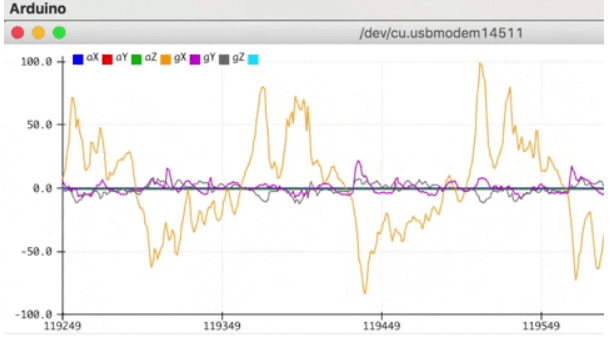
\includegraphics[width=0.5\linewidth]{Images/Nano33BLESense/IMUData}
%	\caption{IMU (Inertial Measurement Unit) Gesture Data} 
%	\label{IMU Sensor Capture Data}
%\end{figure}
%
%The another possibility for detecting gesture is to use the APDS9960 sensor, it can also detect the gesture by moving the hand in front of it. It has also some limitation, it will not detect any gesture above 15 mm distance from the sensor.

%todo GitLab\ToDo\TinyML
% TinyML Seite 222


